
% ===========================================================================
% file: vignette.rnw
% description: 
% requires: 
% author: Sahil Shah <sahil.shah@u.northwestern.edu>
% ==========================================================================

% LaTeX preamble and Top matter ----------------------------------------------

\documentclass[11pt]{article}
\usepackage[margin=0.9in]{geometry}
\usepackage{graphicx, amsmath, url,courier,array,csquotes}

\usepackage{Sweave}
\setkeys{Gin}{width=1.0\textwidth}
\graphicspath{{./}{figs/}}

\usepackage{hyperref}


%http://stackoverflow.com/questions/8902679/getting-sweave-code-chunks-inside-some-framed-box

\DefineVerbatimEnvironment{Sinput}{Verbatim} {xleftmargin=2em,
                                              frame=single}
\DefineVerbatimEnvironment{Soutput}{Verbatim}{xleftmargin=2em,
                                              frame=single}


\begin{document}

% =============================================================================

\title{\vspace{-1cm}The GeneSurrounder package Vignette}

\author{Sahil Shah and Rosemary Braun 
	   \href{mailto:rbraun@northwestern.edu}{<\texttt{rbraun@northwestern.edu}>}}

\date{\today}

\maketitle

% ----------------------------------------------------------------------------

\section*{Availability}  %------------------------------------------------

The \texttt{GeneSurrounder} package and its documentation are available on GitHub at 
\url{https://github.com/sahildshah1}. 


\section*{Introduction}  %------------------------------------------------

The \texttt{GeneSurrounder} package implements the method we previously developed~\cite{SHAH2017}
to identify disease-associated genes from expression data and an independent
network model of cellular interactions. We developed GeneSurrounder to find the genes
with neighbors on the network that are differentially expressed (with the
magnitude of the differential expression decreasing with distance from the
putative disease gene) and have correlated expression with the putative disease
gene. Since the differential expression of the neighbors of a putative disease
gene does not depend on their association with that gene, our algorithm consists
of two tests that are run independently of each other 
(Table~\ref{tab:procedure-sphere}, Table~\ref{tab:procedure-decay}). Their results
are then combined to determine if the putative disease gene is a central
candidate disease gene.

\section*{Example} %------------------------------------------------

In order to illustrate our method, we apply our algorithm  to one study  of
high-vs-low grade ovarian cancer  from the publicly available and curated
collection curatedOvarianData (GEO accession GSE14764)~\cite{Ganzfried2013}. We
have  constructed the global network model from KEGG
pathways~\cite{Kanehisa2008}.


\subsection*{Load Data Set} % --------------------------------------------


Our algorithm uses the correlation between the expression of the genes, their
differential expression, and their distances on the global network. 


\begin{Schunk}
\begin{Sinput}
> load("../../data/CurOvGradeKEGGnets.RData")
> load("../../data/largestCompKEGGigraph.RData")
> 
\end{Sinput}
\end{Schunk}


%figures-illustration.rnw but compute p-values instead of load 2016-04-06/geneNIDG.GSE14764.RData
%follow back geneNIDG.GSE14764 in 2016-04-06 in study.R etc to compute p-values

%<<fig=FALSE,echo=TRUE,width=11.43,height=6.71>>=

% # # GSE14764 -------------------------------------------------------------------
% # load("../../data/CurOv_RankCorMatrix_GSE14764_eset.RData")
% # load('../../data/CurOv_tStatistics.RData')

% # # LCC KEGGG -----------------------------------------------------------------
% # load("../../data/LCCKEGG_ShortestDistMatrix.RData")

% @


\subsection*{Source Functions} % ------------------------------------------

The functions that implement our method have to be sourced. The \texttt{Observed.SI,
Resample.SI,SumAbsCor} functions implement the \textit{Sphere of Influence} procedure
and the \texttt{Resample.DecayDE, Observed.DecayDE} functions implement the 
\textit{Decay of Differential Expression} procedure. The \texttt{geneNIDG}
function calls these functions. 


\begin{Schunk}
\begin{Sinput}
> library(pcaPP)
> library(igraph) # load largestCompKEGGigraph
> library(limma) #calcGeneStats()
> library(metap) #pFisher sumlog()
> source("../../R/calcCorMatrix.R")
> source("../../R/calcGeneTStats.R")
> source("../../R/calcAllPairsDistances.R")
> source("../../R/Observed.SI.R")
> source("../../R/Resample.SI.R")
> source("../../R/SumAbsCor.R")
> source("../../R/Resample.DecayDE.R")
> source("../../R/Observed.DecayDE.R")
> source("../../R/geneNIDG.R")
> 
\end{Sinput}
\end{Schunk}




\subsection*{Apply Functions to Data} % -----------------------------------



The correlation between the expression of the genes is calculated.


\begin{Schunk}
\begin{Sinput}
> CurOv_RankCorMatrix_GSE14764_eset <- 
+ calcCorMatrix(exprMatrix = CurOvGradeKEGGnets[["GSE14764_eset"]]$expr,
+ 			  corMethod = "spearman",
+ 			  exprName = paste("CurOvGradeKEGGnets$","GSE14764_eset",sep=""))
> 
\end{Sinput}
\end{Schunk}

% ---------------------------------------------------------------------------


The observed and resampled differential expression of the genes is calculated. 

\begin{Schunk}
\begin{Sinput}
> # List of observed (vector) and resampled (resampling by gene matrix) t statistics
> 
> intersectGeneNames = intersect(rownames(CurOvGradeKEGGnets[[2]]$expr),
+ 							   V(largestCompKEGGigraph)$name)
> expr = CurOvGradeKEGGnets[["GSE14764_eset"]]$expr
> classLabels = CurOvGradeKEGGnets[["GSE14764_eset"]]$grade
> #I can reduce the number of t tests by reducing the expr matrix to 
> #only genes that are on the network.
> reducedExpr = expr[intersectGeneNames,]
> geneTStats = calcGeneTStats(reducedExpr,
+ 							classLabels,
+ 							numResamples = 1000)
> 
\end{Sinput}
\end{Schunk}

% ---------------------------------------------------------------------------

The distances on the global network are calculated.


\begin{Schunk}
\begin{Sinput}
> CompKEGG_ShortestDistMatrix <- 
+ calcAllPairsDistances(network = largestCompKEGGigraph,
+ 					     directionPaths="all",
+ 					     weightVector = NULL,
+ 					     networkName = "largestCompKEGGigraph")
> 
\end{Sinput}
\end{Schunk}



In this example, MCM2 (KEGG ID: hsa:4171) is the candidate disease gene. 

\begin{Schunk}
\begin{Sinput}
> genes.assayedETnetwork <- intersect(
+ 	rownames(CurOv_RankCorMatrix_GSE14764_eset),
+ 	rownames(CompKEGG_ShortestDistMatrix))
> gene.id <- "hsa:4171"
> 
\end{Sinput}
\end{Schunk}


% ---------------------------------------------------------------------------



The Sphere of Influence and Decay of Differential Procedures are run.


\begin{Schunk}
\begin{Sinput}
> geneNIDG.hsa4171 <-  geneNIDG(
+ 	gene.id = gene.id,
+ 	distance.matrix = CompKEGG_ShortestDistMatrix,
+ 	cor.matrix = CurOv_RankCorMatrix_GSE14764_eset,
+ 	geneStats.observed = geneTStats$observed,
+ 	perm.geneStats.matrix = geneTStats$resampled,
+ 	num.Sphere.resamples = 1000,
+ 	diameter = 34,
+ 	genes.assayedETnetwork = genes.assayedETnetwork)
> 
> 
\end{Sinput}
\end{Schunk}

% ---------------------------------------------------------------------------


The evidence from both procedures is combined. 


\begin{Schunk}
\begin{Sinput}
> p.Fisher <- vapply( 1:34, function(index){
+ 
+ 	x <- sumlog( c(geneNIDG.hsa4171$p.Decay[index],
+ 			geneNIDG.hsa4171$p.Sphere[index]) )
+ 
+ 	return(x$p)
+ 
+ 
+ },
+ numeric(1) )
> geneNIDG.hsa4171 <- cbind(geneNIDG.hsa4171,p.Fisher)
> 
\end{Sinput}
\end{Schunk}
% ---------------------------------------------------------------------------




\subsection*{Description of the Output} % ---------------------------------



Our method outputs a data frame. 


\begin{Schunk}
\begin{Sinput}
> str(geneNIDG.hsa4171)
\end{Sinput}
\begin{Soutput}
'data.frame':	34 obs. of  8 variables:
 $ gene.id       : Factor w/ 1 level "hsa:4171": 1 1 1 1 1 1 1 1 1 1 ...
 $ radius        : int  1 2 3 4 5 6 7 8 9 10 ...
 $ size          : num  9 14 17 46 169 ...
 $ observed.tau_b: num  NaN -0.0156 -0.046 -0.4233 -0.0916 ...
 $ p.Decay       : num  1 0.502 0.433 0.003 0.117 0.029 0.7 0.211 0.124 0.12 ...
 $ observed.cor  : num  3.29 6.2 7.45 14.36 39.42 ...
 $ p.Sphere      : num  0.001 0.000999 0.000999 0.000999 0.000999 ...
 $ p.Fisher      : num  7.91e-03 4.31e-03 3.78e-03 4.11e-05 1.18e-03 ...
\end{Soutput}
\begin{Sinput}
> 
> 
\end{Sinput}
\end{Schunk}

% =======================================================================

We plot the results against every radius.

\begin{Schunk}
\begin{Sinput}
> source("../../R/plotRadiusVS.R")
> plotRadiusVS(geneNIDG.hsa4171)
> 
\end{Sinput}
\end{Schunk}
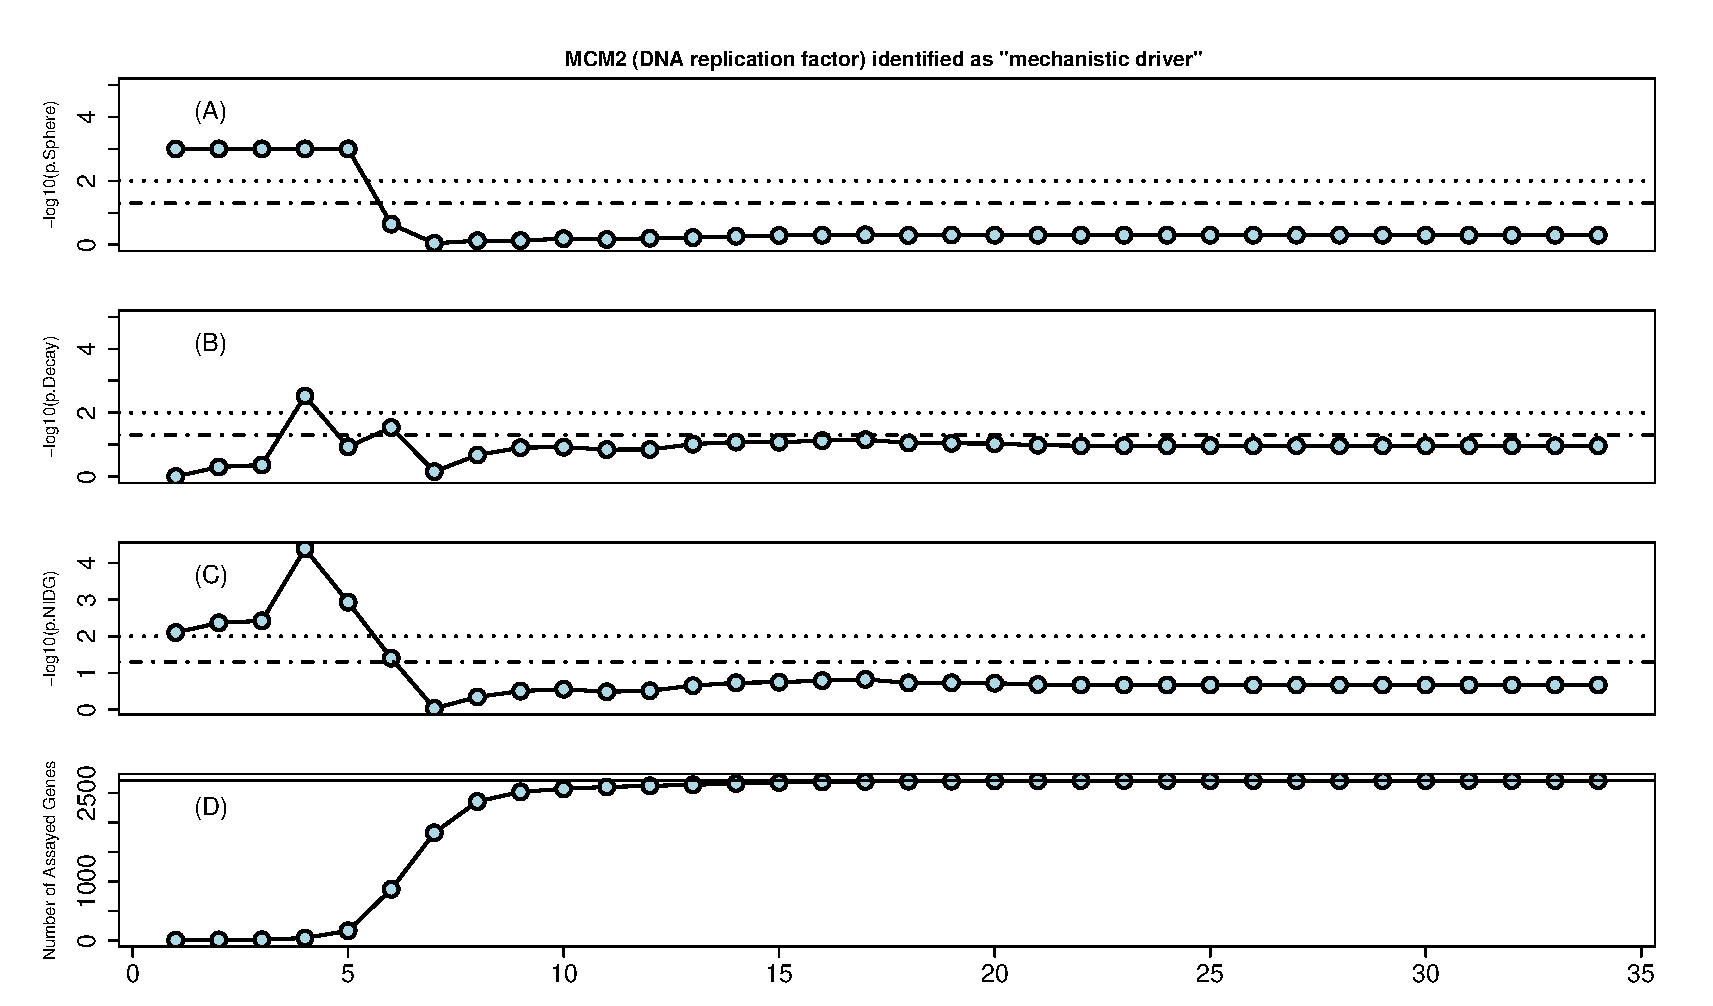
\includegraphics{vignette-main-010}



% \SweaveInput{vignette-radiusVSplots.rnw}


% =========================================================================

% \clearpage

% \subsection*{Tables}

% \SweaveInput{tables-sphere.rnw}

% \SweaveInput{tables-decay.rnw}



% Bibliography -------------------------------------------------------------

\clearpage
\bibliographystyle{unsrt}
% comma separated list:
\bibliography{main}




\end{document}
